\documentclass{article}
\usepackage{amsthm}
\usepackage{graphicx}
\usepackage{ctex}
\usepackage{amsmath}
\usepackage{amssymb} % 添加 amssymb 以支持更多符号
\usepackage{amsfonts}
\usepackage{tikz} % 文氏图
\usetikzlibrary{shapes.geometric, arrows.meta, positioning}
\title{离散数学作业\_2}
\author{李云浩 241880324}
\date{\today}
\begin{document}
\maketitle
\section{pp.3-5}

\subsection{T5}
(a) F \quad (b) F \quad (c) F \quad (d) T \quad (e) F \quad (f) F

\subsection{T10}
(a)(e)

\subsection{T16}
(a) T \quad (b) T \quad (c) T \quad (d) T \quad (e) T

\subsection{T30}
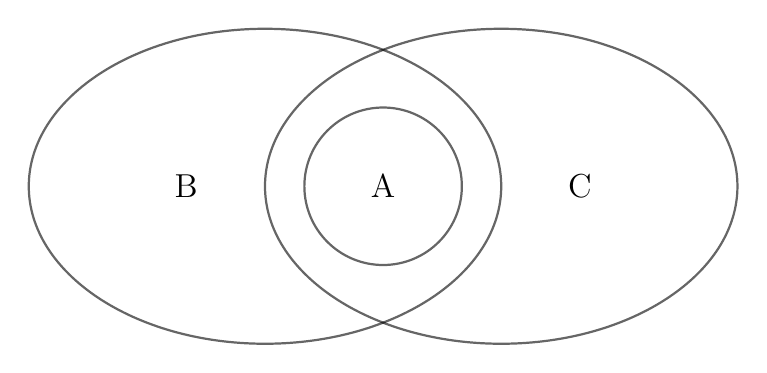
\begin{tikzpicture}[
    set/.style={
        ellipse, 
        draw=black, 
        thick, 
        minimum width=2cm, 
        minimum height=2cm,
        opacity=0.6
    },
    label/.style={font=\large, inner sep=2pt}
]

% 定义三个椭圆集合的位置
\node[set, minimum width = 6cm, minimum height = 4cm, label={[label]B}] (B) at (0,0) {};
\node[set, minimum width = 6cm, minimum height = 4cm, label={[label]C}] (C) at (3,0) {};
\node[set, label={[label]A}] (A) at (1.5,0) {};

% 添加公式标签
\node[label] at (1.5, 0) {A};
\node[label] at (-1, 0) {B};
\node[label] at (4, 0) {C};

\end{tikzpicture}

\subsection{T31}
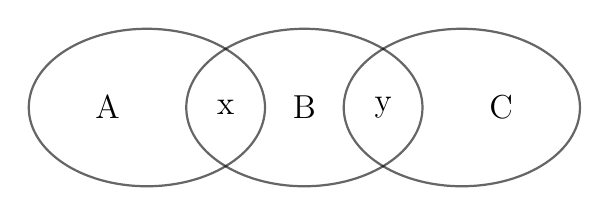
\begin{tikzpicture}[
    set/.style={
        ellipse, 
        draw=black, 
        thick, 
        minimum width=3cm, 
        minimum height=2cm,
        opacity=0.6
    },
    label/.style={font=\large, inner sep=2pt}
]

\node[set, label = {[label] A}] (A) at (0,0){};
\node[set, label = {[label] B}] (B) at (2,0){};
\node[set, label = {[label] C}] (C) at (4,0){};

\node[label] at (1, 0) {x};
\node[label] at (3, 0) {y};
\node[label] at (-0.5, 0) {A};
\node[label] at (2, 0) {B};
\node[label] at (4.5, 0) {C};

\end{tikzpicture}

\subsection{T34}
由$A \subseteq B$,可知对于$\forall x \in A$都有$x \in B$。同理,
由$B \subseteq C$,可知对于$\forall y \in B$都有$y \in B$。因此可推得:
$\forall x \in A$都有$x \in C$,即$A \subseteq C$。证毕。

由文氏图可进一步验证该结果:

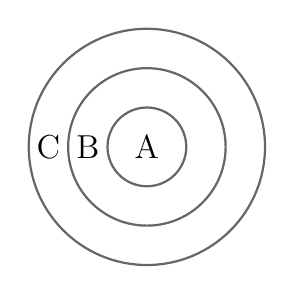
\begin{tikzpicture}[
    set/.style={
        ellipse, 
        draw=black, 
        thick, 
        minimum width=1cm, 
        minimum height=1cm,
        opacity=0.6
    },
    label/.style={font=\large, inner sep=2pt}
]

\node[set, label = {[label] A}] (A) at (0,0){};
\node[set, minimum width = 2cm, minimum height = 2cm, label = {[label] B}] (B) at (0,0){};
\node[set, minimum width = 3cm, minimum height = 3cm, label = {[label] C}] (C) at (0,0){};

\node[label] at (0,0) {A};
\node[label] at (-0.75, 0) {B};
\node[label] at (-1.25, 0) {C};

\end{tikzpicture}

\subsection{T36}
因为集合$B$是由集合$A$的所有元素以及一个额外的元素组成的,那么
$A$的所有子集$S_1, S_2, \dots, S_n$同时也是$B$的子集,有$n$个。同时,
对于$A$的每个子集,额外加上那个$B$的特有元素,形成的新集合也是$B$的子集,
并且与之前的子集不会重复,有$n$个。故$B$的子集个数为:$n + n = 2n$

\section{pp.10-14}
\subsection{T1}\noindent
$(a) A \cup B  = \{a, b, c, d, e, f, g\} \quad (b) B \cup C = \{a, c, d, e, f, g\} \quad (c) A \cap C = \{a, c\}$\\
$(d) B \cap D = \{f\}\quad (e) (A \cup B) - C = \{b, d, e, g\} \quad (f) A - B = \{a, b, c\}$\\ 
$(g) \overline{A} = \{d, e, f, h, k\} \quad (h) A \oplus B = \{a, b, c, d, e, f\} \quad (i) A \oplus C = \{b, g, f\}$\\
$(j) (A \cap B) - C = \{g\}$

\subsection{T6}\noindent
$(a) A - B = \{1, 6, 8\} \quad (b) B - A = \{5, 9\} \quad (c) C - D = \{1, 2, 3, 4\}$\\
$(d) \overline{C} = \{5, 6, 7, 8, 9\} \quad (e)\overline{A} = \{3, 5, 7, 9\} \quad (f) A \oplus B = \{1, 5, 6, 8, 9\}$\\
$(g) C \oplus D = \{1, 2, 3, 4, 7, 8\} \quad (h) B \oplus C = \{1, 3, 5, 9\}$

\subsection{T10}\noindent
$(a) \overline{A} \cap \overline{B} = \{b, d, h\} \quad (b) \overline{B} \cup \overline{C} = U \quad (c) \overline{A \cup A} = \{b, d, e, h\}$\\
$(d) \overline{C \cap C} = \{a, c, d, e, f, g\} \quad (e) A \oplus B = \{c, e, f, g\} \quad (f) B \oplus C = \{a, b, e, h\}$

\subsection{T23}
定理三:
\[
    |A \cup B \cup C| = |A| + |B| + |C| - |A \cap B| - |B \cap C| - |A \cap C| + |A \cap B \cap C|
\]

因为:$A = \{1, 2, 3, 4, 5, 6\}, B = \{2, 4, 7, 8, 9\}, C = \{1, 2, 4, 7, 10, 12\}$,则
\(|A| = 6, |B| = 5, |C| = 6, |A \cup B \cup C| = 11, |A \cap B| = 2, |B \cap C| = 3, 
|A \cap C| = 3, |A \cap B \cap C| = 2\)

所以:\(|A| + |B| + |C| - |A \cap B| - |B \cap C| - |A \cap C| + |A \cap B \cap C|
= 6 + 5 + 6 - 2 - 3 - 3 + 2 = 11 = |A \cup B \cup C|\),证毕。

\subsection{T24}
因为:$A = \{1, 2, 3, 4, 5, 6, 7\}, \quad B = \{2, 3, 4\}, \quad C = \{-3, -2, -1, 0, 1, 2, 3\}$,则
\(|A| = 7, |B| = 3, |C| = 7, |A \cap B| = 3, |B \cap C| = 2, |A \cap C| = 3, |A \cap B \cap C| = 2,
|A \cup B \cup C| = 11\)

所以:\(|A| + |B| + |C| - |A \cap B| - |B \cap C| - |A \cap C| + |A \cap B \cap C|
= 7 + 3 + 7 - 3 - 2 - 3 + 2 = 11 = |A \cup B \cup C|\),证毕。

\subsection{T34}
(a) 可能为真,可能为假 \quad (b) 可能为真,可能为假 \quad (c) 可能为真,可能为假 \quad
(d) 可能为真,可能为假 \quad (e) 可能为真,可能为假 \quad (f) 可能为真,可能为假

\subsection{T36}
(a) 真 \quad (b) 可能为真,可能为假 \quad (c) 可能为真,可能为假 \quad (d) 假 \quad
(e) 真 \quad (f) 真

\subsection{T39}
假设$x \in A \cap B$,那么$x$属于$A$,所以$A \cap B \subseteq A$。

\section{pp.19-21}
\subsection{T19}
公式:$a_n = 3n - 2$

观察序列可知,每两项之间差值为二,且第一项为$1$。即:$a_n = a_{n - 1} + 3, a_1 = 1$。
由递推关系可证:
\begin{align*}
    a_n &= a_{n - 1} + 3\\
    &= a_{n - 2} + 2 \times 3\\
    &\ \,\vdots\\
    &= a_1 + (n - 1) \times 3\\
    &= 3n - 2\\
\end{align*}

\subsection{T20}
公式:$a_n = (\frac{1}{2})^{n - 1}$

观察序列可知,后一项为前一项乘$\frac{1}{2}$,且第一项为$1$。即:$a_n = \frac{a_{n-1}}{2}, a_1 = 1$。
由递推关系可证:
\begin{align*}
    a_n &= \frac{1}{2} a_{n - 1}\\
    &= (\frac{1}{2})^2 a_{n - 2}\\
    &\ \, \vdots\\
    &= (\frac{1}{2})^{n - 1} a_1\\
    &= (\frac{1}{2})^{n - 1}\\
\end{align*}

\subsection{T22}
公式:$a_n = \frac{15 + \sqrt{5}}{10}(\frac{1+\sqrt{5}}{2})^n + \frac{15 - \sqrt{5}}{10}(\frac{1-\sqrt{5}}{2})^n$

\subsection{T25}
(a)属于 \quad (b) 不属于 \quad (c) 属于 \quad (d) 属于 \quad (e) 不属于 \quad (f) 不属于

\subsection{T29}
\begin{align*}
    (A \oplus B) \oplus C &= (f_A + f_B - 2f_Af_B) \oplus C\\
    &= f_A + f_B - 2f_Af_B + f_C - 2(f_A + f_B - 2f_Af_B)f_C\\
    &= f_A + f_B + f_C - 2f_Af_B - 2f_Af_C - 2f_Bf_C + 4f_Af_Bf_C\\
    &= f_B + f_C - 2f_Bf_C + f_A - 2(f_b + f_C - 2f_Bf_C)f_A\\
    &= (f_B + f_C - 2f_Bf_C) \oplus A\\
    &= (B \oplus C) \oplus A\\
    &= A \oplus (B \oplus C)\\
\end{align*}证毕。

\subsection{T32}\noindent
(a) $(a^* b \lor c) = \{ab, ac, aab, aac, \dots\}$,属于\\
(b) $(ab)^*c = \{abc, ababc, \dots\}$,不属于\\
(c) $(a^* \lor b)c^* = \{ac, bc, \dots,  a \dots ac \dots c, bc \dots c\}$,属于

\subsection{T34}
(a)$(p \lor q)rq^* = \{prq, qrq, prqq, qrqq, \dots \}$\\
(b)$p(qq)^*r = \{pqqr, pqqqqr, \dots ,pqq \dots qqr\}$
\subsection{T37}
因为8是一个$S^-$数,由(3)可知,因为1是8的倍数,因此1也是一个$S^-$数。因此1的所有倍数
都是$S^-$数,所以$S^-$数集合即整数集$\mathbf{Z}$。
\section{pp.31-33}
\subsection{T24}
\begin{itemize}
    \item 因为 $a \mid b$,所以对于$\forall m \in \mathbf{Z}$有:$a \mid mb$。
    \item 同理:因为$a \mid c$,所以对于$\forall n \in \mathbf{Z}$有:$a \mid nc$
    \item 由于$a \mid mb, a \mid nc$,因此$a \mid mb + nc$。
\end{itemize}
证毕。
\subsection{T25}
$p$有且只有$p$和$1$两个因数并且$p \nmid a$,则$p$不是$a$的因数,所以$GCD(a, p) = 1$\\
$p \mid ab$以及$p \mid p$,因此$p \mid sab, p \mid tpb$,所以$p \mid sab + tpb$。

\subsection{T26}
因为$GCD(a, c) = 1$,所以由定理4可知:有某个整数s 和 t,使得 $1 = sa + tc$,于是$b = sab + tcb$
因为$c \mid ab, c \mid c$,所以$c \mid sab, c \mid tcb$,所以$c \mid sab + tcb$,所以$c \mid b$。证毕。

\subsection{T27}
因为$GCD(a,c) = 1$,所以a和c互质。因为$a \mid m, c \mid m$,因此,m拥有因数a,c。因为a和c互质,所以$ac \mid m$。

\subsection{T28}
因为$d = GCD(a,b)$,所以$\exists x,y \in \mathbf{Z}, a = dx, b = yd, GCD(x,y) = 1$。
又因为$a \mid b, c\mid d$,所以$\exists m,n \in \mathbf{Z}, b = am, d = cn$。
所以:$yd = am = dmx, a = dx = cnx$,所以$ac = c^2nx, bd = yd^2 = yc^2n^2$。
又因为$y = mx$,所以$bd = c^2n^2mx$。因此$bd = nmac$,所以$ac \mid bd$,证毕。

\subsection{T29}
因为$c \mid ca,c \mid cb$,所以$c$显然为$ca,cb$的一个公因数,所以$GCD(ca,cb) = cGCD(a,b)$

\section{pp.41-44}
\subsection{T6}
(a) 
\begin{align*}
A(BD) &= 
\begin{bmatrix} 
    2 & 1 & 3\\ 
    4 & 1 & -2\\
\end{bmatrix} 
\left(
\begin{bmatrix} 
    0 & 1\\
    1 & 2\\ 
    2 & 3\\
\end{bmatrix}
\begin{bmatrix}
    -3 & 2\\
    4 & 1\\
\end{bmatrix}
\right)\\
&= \begin{bmatrix} 
    2 & 1 & 3\\ 
    4 & 1 & -2\\
\end{bmatrix} 
\begin{bmatrix}
    4 & 1\\
    5 & 4\\
    6 & 7\\
\end{bmatrix}\\
&=
\begin{bmatrix}
    31 & 27\\
    9 & -6\\
\end{bmatrix}
\end{align*}
\begin{align*}
    (AB)D &=
    \left(
    \begin{bmatrix}
        2 & 1 & 3\\
        4 & 1 & -2\\
    \end{bmatrix}
    \begin{bmatrix}
        0 & 1\\
        1 & 2\\
        2 & 3\\
    \end{bmatrix}
    \right)
    \begin{bmatrix}
        -3 & 2\\
        4 & 1\\
    \end{bmatrix}\\
    &=
    \begin{bmatrix}
        7 & 13\\
        -3 & 0\\
    \end{bmatrix}
    \begin{bmatrix}
        -3 & 2\\
        4 & 1\\
    \end{bmatrix}\\
    &=
    \begin{bmatrix}
        31 & 27\\
        9 & -6\\
    \end{bmatrix}
\end{align*}

(b)
\begin{align*}
    A(C+E) &= 
    \begin{bmatrix}
        2 & 1 & 3\\
        4 & 1 & -2\\
    \end{bmatrix}
    \left(
        \begin{bmatrix}
            1 & -2 & 3\\
            4 & 2 & 5\\
            3 & 1 & 2\\
        \end{bmatrix}
        + 
        \begin{bmatrix}
            3 & 2 & -1\\
            5 & 4 & -3\\
            0 & 1 & 2\\
        \end{bmatrix}
    \right)\\
    &= 
    \begin{bmatrix}
        2 & 1 & 3\\
        4 & 1 & -2\\
    \end{bmatrix}
    \begin{bmatrix}
        4 & 0 & 2\\
        9 & 6 & 2\\
        3 & 2 & 4\\
    \end{bmatrix}\\
    &=
    \begin{bmatrix}
        26 & 12 & 18\\
        19 & 2 & 2\\
    \end{bmatrix}
\end{align*}
\begin{align*}
    AC+AE &= 
    \begin{bmatrix}
        2 & 1 & 3\\
        4 & 1 & -2\\
    \end{bmatrix}
    \begin{bmatrix}
        1 & -2 & 3\\
        4 & 2 & 5\\
        3 & 1 & 2\\
    \end{bmatrix}
    +
    \begin{bmatrix}
        2 & 1 & 3\\
        4 & 1 & -2\\
    \end{bmatrix}
    \begin{bmatrix}
        3 & 2 & -1\\
        5 & 4 & -3\\
        0 & 1 & 2\\
    \end{bmatrix}\\
    &=
    \begin{bmatrix}
        15 & 1 & 17\\
        2 & -8 & 13\\
    \end{bmatrix}
    +
    \begin{bmatrix}
        11 & 11 & 1\\
        17 & 10 & -11\\
    \end{bmatrix}\\
    &=
    \begin{bmatrix}
        26 & 12 & 18\\
        19 & 2 & 2\\
    \end{bmatrix}
\end{align*}
(c)
\begin{align*}
    FD+AB &=
    \begin{bmatrix}
        -2 & 3\\
        4 & 5\\
    \end{bmatrix}
    \begin{bmatrix}
        -3 & 2\\
        4 & 1\\
    \end{bmatrix}
    +
    \begin{bmatrix}
        2 & 1 & 3\\
        4 & 1 & -2\\
    \end{bmatrix}
    \begin{bmatrix}
        0 & 1\\
        1 & 2\\
        2 & 3\\
    \end{bmatrix}\\
    &=
    \begin{bmatrix}
        18 & -1\\
        8 & 13\\
    \end{bmatrix}
    +
    \begin{bmatrix}
        7 & 13\\
        -3 & 0\\
    \end{bmatrix}\\
    &=
    \begin{bmatrix}
        25 & 12\\
        5 & 13\\
    \end{bmatrix}
\end{align*}

\subsection{T9}
(a)
\begin{align*}
    A^T(D+F) &=
    \begin{bmatrix}
        2 & 4\\
        1 & 1\\
        3 & -2\\
    \end{bmatrix}
    \left(
    \begin{bmatrix}
        -3 & 1\\
        4 & 1\\
    \end{bmatrix}
    +
    \begin{bmatrix}
        -2 & 3\\
        4 & 5\\
    \end{bmatrix}
    \right)\\
    &=
    \begin{bmatrix}
        2 & 4\\
        1 & 1\\
        3 & -2\\
    \end{bmatrix}
    \begin{bmatrix}
        -5 & 4\\
        8 & 6\\
    \end{bmatrix}\\
    &=
    \begin{bmatrix}
        22 & 32\\
        3 & 10\\
        -31 & 0\\
    \end{bmatrix}
\end{align*}

(b)
\begin{align*}
    (BC)^T &=
    \left(
    \begin{bmatrix}
        0 & 1\\
        1 & 2\\
        2 & 3\\
    \end{bmatrix}
    \begin{bmatrix}
        1 & -2 & 3\\
        4 & 2 & 5\\
        3 & 1 & 2\\
    \end{bmatrix}
    \right)^T\\
    &= \text{无法计算}
\end{align*}

\begin{align*}
    C^TB^T &=
    \left(
        \begin{bmatrix}
            1 & 4 & 3\\
            -2 & 2 & 1\\
            3 & 5 & 2\\
        \end{bmatrix}
        \begin{bmatrix}
            0 & 1 & 2\\
            1 & 2 & 3\\
        \end{bmatrix}
    \right)\\
    &= \text{无法计算}
\end{align*}

(c)
\begin{align*}
    (B^T+A)C &=
    \left(
    \begin{bmatrix}
        0 & 1 & 2\\
        1 & 2 & 3\\
    \end{bmatrix}
    +
    \begin{bmatrix}
        2 & 1 & 3\\
        4 & 1 & -2\\
    \end{bmatrix}
    \right)
    \begin{bmatrix}
        1 & -2 & 3\\
        4 & 2 & 5\\
        3 & 1 & 2\\
    \end{bmatrix}\\
    &=
    \begin{bmatrix}
        2 & 2 & 5\\
        5 & 3 & 1\\
    \end{bmatrix}
    \begin{bmatrix}
        1 & -2 & 3\\
        4 & 2 & 5\\
        3 & 1 & 2\\
    \end{bmatrix}\\
    &=
    \begin{bmatrix}
        25 & 5 & 26\\
        20 & -3 & 32\\
    \end{bmatrix}
\end{align*}

(d)
\begin{align*}
    (D^T+E)F &=
    \left(
        \begin{bmatrix}
            -3 & 4\\
            2 & 1\\
        \end{bmatrix}
        +
        \begin{bmatrix}
            3 & 2 & -1\\
            5 & 4 & -3\\
            0 & 1 & 2\\
        \end{bmatrix}
    \right)
    \begin{bmatrix}
        -2 & 3\\
        4 & 5\\
    \end{bmatrix}\\
    &= \text{无法计算}
\end{align*}

\subsection{T16}
(a) 假设$A$的第$i$行全为0,那么在计算$AB$时,$AB$的第$i$行元素是$A$的第$i$行元素
与$B$的各列元素相乘所得,由于$A$的第$i$行全为0,故$AB$的第$i$行元素也全为0。

(b)如果$B$有一列全为0,即$B^T$有一行全为零,由(a)可知,$B^TA^T$也会有一行元素全为0。
因为$B^TA^T = (AB)^T$,因此$(AB)^T$有一行全为零,即$AB$有一列全为0。

\subsection{T17}
对于矩阵$B^TA^T$,其第$j$行的元素为$B^T$的第$j$行元素与$A^T$的各列元素相乘所得,即$(B^T)_jA^T$,
这里的$(B^T)j$是$B^T$的第$j$行。
因为$B^TA^T = (AB)^T$,所以即有$AB$的第$j$列等于$AB_j$,这里的$B_j$是$B$的第$j$列。

\subsection{T23}
(a) 证明:$(A^T)^T = A$\\
因为$A$是一个$m\times n$矩阵,其元素为$a_{ij}$。那么$A^T$是一个$n \times m$矩阵,其元素为$a_{ji}$。
再次转置后:$(A^T)^T$是一个$m \times n$矩阵,其元素为$a_{ij}$,故$(A^T)^T = A$,证毕。

(b) 证明:$(A + B)^T = A^T + B^T$\\
设$A,B$都是$m \times n$矩阵,其元素分别为$a_{ij}, b_{ij}$,因此$A + B$的元素为$a_{ij} + b_{ij}$。
对$A+B$进行转置,$(A+B)^T$中的元素为$a_{ji} + b_{ji}$。同时,$A^T + B^T$的元素亦为$a_{ji} + b_{ji}$。
因此$(A + B)^T = A^T + B^T$,证毕。

(c) 证明:$(AB)^T = B^TA^T$\\
设$A = (a_{ij})_{m\times l}, B = (b_{ij})_{l \times n}$,则$[(AB)^T]_{ij} = [AB]_{ji}
= a_{j1}b_{1i} + a_{j2}b_{2i} + \dots + a_{jl}b_{li},(i = 1, \dots , m; j = 1, \dots , n)$,
另一方面,$[B^TA^T]_{ij}$是$B^T$的第$i$行与$A^T$的第$j$列对应元素的乘积之和,亦即$B$的第$i$列
与$A$的第$j$行对应元素的乘积之和。于是$(B^TA^T)_{ij} = b_{1i}a_{j1} + b_{2i}a_{j2} + \dots +b_{li}a_{jl}
= [(AB)^T]_{ij}, (i = 1, \dots ,m; j = 1, \dots, n)$.因此$(AB)^T = B^TA^T$,证毕。

\subsection{T29}
因为
\[
(AB)(B^{-1}A^{-1}) = A(BB^{-1})A^{-1} = AEA^{-1} = AA^{-1} = E
\]
\[
(B^{-1}A^{-1})(AB) = B^{-1}(A^{-1}A)B = B^{-1}EB = B^{-1}B = E
\]
所以$AB$可逆,且$(AB)^{-1} = B^{-1}A^{-1}$.
\subsection{T41}
设$A = (a_{ij})_{m \times n}, B = (b_{ij})_{m \times n}, C = (c_{ij})_{m \times n}$。
因此
\begin{align*}
    A \lor (B \lor C) &= (a_{ij})_{m \times n} \lor [(b_{ij})_{m \times n} \lor (c_{ij})_{m \times n}]\\
    &= [a_{ij} \lor (b_{ij} \lor c_{ij})]_{m \times n}\\
    &= [a_{ij} \lor b_{ij} \lor c_{ij}]_{m \times n}\\
    &= [(a_{ij} \lor b_{ij}) \lor c_{ij}]_{m \times n}\\
    &= [(a_{ij})_{m \times n} \lor (b_{ij})_{m \times n}] \lor (c_{ij})_{m \times n}\\
    &= (A \lor B) \lor C\\ 
\end{align*}证毕。

\section{pp.47-49}
\subsection{T24}
$\forall x, y \in \mathbf{Q} \rightarrow (x + y) \in \mathbf{Q}$。
$\forall x \in \mathbf{Q} \rightarrow \frac{x}{2} \in \mathbf{Q}$。
因此$\forall x, y \in \mathbf{Q} \rightarrow \frac{x + y}{2} \in \mathbf{Q}$。封闭性成立。
\subsection{T25}
$\forall x, y \in \mathbf{Q}, \frac{x + y}{2} = \frac{y + x}{2}$,所以$x \square y = y \square x$。交换性成立。

\subsection{T26}
$\forall x,y,z \in \mathbf{Q}, (x \square y) \square z = \frac{\frac{x + y}{2} + z}{2} = \frac{x + y + 2z}{4}$。
$x \square (y \square z) = \frac{x + \frac{y + z}{2}}{2} = \frac\bigtriangledown {2x + y + z}{4}$。
因为$(x \square y) \square z \neq x \square (y \square z)$,因此结合律不满足。

\subsection{T27}
假设存在单位元n,则$\forall x \in \mathbf{Q}, x \square n = x$。因为$x \square n = \frac{x + n}{2}$,
当且仅当$n = x时,x \square n = x$。因此不存在单位元。

\subsection{T28}
由于单位元不存在,故逆元也不存在。

\subsection{T29}
(a) $\forall x, y, w, z \in R$,
\[
\begin{bmatrix}
    x\\
    y
\end{bmatrix}
\bigtriangledown 
\begin{bmatrix}
    w\\
    z
\end{bmatrix}
=
\begin{bmatrix}
    x + w\\
    y + z +1
\end{bmatrix}
\in R^2
\]
因此满足封闭性质。

(b) $\forall x, y, w, z \in R$
\[
\begin{bmatrix}
    x\\
    y
\end{bmatrix}
\bigtriangledown 
\begin{bmatrix}
    w\\
    z
\end{bmatrix}
=
\begin{bmatrix}
    x + w\\
    y + z +1
\end{bmatrix}
\]
\[
    \begin{bmatrix}
        w\\
        z
    \end{bmatrix}
    \bigtriangledown 
    \begin{bmatrix}
        x\\
        y
    \end{bmatrix}
    =
    \begin{bmatrix}
        w + x\\
        z + y +1
    \end{bmatrix}
\]
因为:
\[
    \begin{bmatrix}
        x + w\\
        y + z +1
    \end{bmatrix}
    =
    \begin{bmatrix}
        w + x\\
        z + y +1
    \end{bmatrix}
\]
因此交换性质成立。

(c)$\forall m, n, w, x, y, z \in R$
\[
\begin{bmatrix}
    x\\
    y
\end{bmatrix}
\bigtriangledown
\left(
    \begin{bmatrix}
        w\\
        z
    \end{bmatrix}
    \bigtriangledown
    \begin{bmatrix}
        m\\
        n
    \end{bmatrix}
\right)
=
\begin{bmatrix}
    x\\
    y
\end{bmatrix}
\bigtriangledown
\begin{bmatrix}
    w + m\\
    z + n + 1
\end{bmatrix}
=
\begin{bmatrix}
    x + w + m\\
    y + z + n + 2
\end{bmatrix},
\]
\[
\left(
    \begin{bmatrix}
        x\\
        y
    \end{bmatrix}
    \bigtriangledown
    \begin{bmatrix}
        w\\
        z
    \end{bmatrix}
\right)
\bigtriangledown
\begin{bmatrix}
    m\\
    n
\end{bmatrix}
=
\begin{bmatrix}
    x + w\\
    y + z + 1
\end{bmatrix}
\bigtriangledown
\begin{bmatrix}
    m\\
    n
\end{bmatrix}
=
\begin{bmatrix}
    x + w + m\\
    y + z + m + 2
\end{bmatrix}
\]
结合性质满足
\subsection{T35}
即证:
对于$5 \times 5$的矩阵$A, B$,$comp(A \land B) = compA \lor compB$, 
$comp(A \lor B) = compA \land compB$。

由$comp$的定义可知,$compA = \overline{A}$
令$C = comp(A \land B)$,即$\overline{C} = A \land B$。所以
\[
\overline{c_{ij}} =
\begin{cases}
    1 & a_{ij} = b_{ij} = 1\\
    0 & else
\end{cases}
\Rightarrow 
c_{ij} = 
\begin{cases}
    1 & (a_{ij} = 0) \lor (b_{ij} = 0)\\
    0 & else
\end{cases}
\]
$compA \lor compB = \overline{a_{ij}} \lor \overline{b_{ij}}$ 
\[
\overline{a_{ij}} \lor \overline{b_{ij}} = 
\begin{cases}
    1 & (a_{ij} = 0) \lor (b_{ij} = 0)\\
    0 & else
\end{cases}
\]
因此$c_{ij} = \overline{a_{ij}} \lor \overline{b_{ij}}$,
所以$C = comp(A \land B) = compA \lor compB$。

令$D = comp(A \lor B)$,即$\overline{D} = A \lor B$。
所以
\[
\overline{d_{ij}}=
\begin{cases}
    1 & (a_{ij} = 1) \lor (b_{ij} = 1)\\
    0 & else
\end{cases}
\Rightarrow
d_{ij} = 
\begin{cases}
    1 & a_{ij} = b_{ij} = 0\\
    0 & else
\end{cases}
\]
$compA \land compB = \overline{a_{ij}} \land \overline{b_{ij}}$
\[
\overline{a_{ij}} \land \overline{b_{ij}}
\begin{cases}
    1 & a_{ij} = b_{ij} = 0\\
    0 & else
\end{cases}
\]
因此$d_{ij} = \overline{a_{ij}} \land \overline{b_{ij}}$,所以$D = comp(A \lor B) = compA \land compB$。
证毕。
\end{document}